% BGIN Block 15 — sponsorship / participation deck, Bitcoin Core edition
% Derived from main_slides_BGIN15_project11.pdf (BGIN, 3 Sep 2026); same structure,
% re-angled for the Bitcoin Core and Bitcoin infrastructure community around the
% PQC Migration track and the METI/NEDO-hosted PQC Migration Prize.
% Build: latexmk -pdf main_slides_BGIN15_bitcoin_core.tex
\documentclass[aspectratio=169,10pt]{beamer}
\usepackage[utf8]{inputenc}
\usepackage[T1]{fontenc}
\usepackage{helvet}
\renewcommand{\familydefault}{\sfdefault}
\usepackage{booktabs}
\usepackage{array}
\usepackage{graphicx}
\usepackage{fontawesome5}
\usepackage{tikz}
\usepackage{hyperref}

% ---------- look: dark title bar, white body, grey footer (as in the original) ----------
\usetheme{default}
\usecolortheme{default}
\definecolor{bar}{RGB}{25,25,29}
\definecolor{ink}{RGB}{35,35,40}
\definecolor{soft}{RGB}{110,110,118}
\definecolor{boxbg}{RGB}{242,242,244}
\definecolor{btc}{RGB}{242,169,0}
\setbeamercolor{normal text}{fg=ink}
\setbeamercolor{structure}{fg=bar}
\setbeamercolor{frametitle}{bg=bar,fg=white}
\setbeamercolor{block title}{bg=bar,fg=white}
\setbeamercolor{block body}{bg=boxbg,fg=ink}
\setbeamertemplate{navigation symbols}{}
\setbeamertemplate{itemize item}{\color{bar}\faAngleRight}
\setbeamertemplate{itemize subitem}{\color{soft}\textendash}
\setbeamertemplate{enumerate item}{\colorbox{bar}{\color{white}\scriptsize\insertenumlabel}}
\setbeamerfont{frametitle}{series=\bfseries,size=\large}
\setbeamertemplate{frametitle}{%
  \vskip-2pt\begin{beamercolorbox}[wd=\paperwidth,ht=8mm,dp=2.5mm,leftskip=6mm]{frametitle}%
  \usebeamerfont{frametitle}\insertframetitle\end{beamercolorbox}}
\setbeamertemplate{footline}{%
  \begin{beamercolorbox}[wd=\paperwidth,ht=5mm,dp=2mm,leftskip=6mm,rightskip=6mm]{normal text}%
  \tiny\color{soft}\raisebox{-1.2pt}{
\includegraphics[height=3.2mm]{bgin_mark.png}}\hspace{1.2mm}%
  BGIN Block 15 --- PQC Migration Track \textperiodcentered{} Bitcoin Core edition\hfill
  Washington, D.C. / Oct 2026\quad\insertframenumber\end{beamercolorbox}}
\newcommand{\why}[1]{\vspace{1.5mm}{\small\color{bar}\faLink~\textbf{Why it matters:} #1}}
\newcommand{\lead}[1]{\begin{beamercolorbox}[wd=\textwidth,sep=2.5mm,rounded=false]{block body}\small #1\end{beamercolorbox}\vspace{2mm}}
\newcommand{\pillar}[2]{\begin{minipage}[t]{0.31\textwidth}\colorbox{bar}{\parbox{\dimexpr\linewidth-2\fboxsep}{\color{white}\textbf{#1}}}\\[1mm]{\small #2}\end{minipage}}
\hypersetup{colorlinks,urlcolor=bar,linkcolor=ink}

\title{Invitation to BGIN Block \#15}
\subtitle{PQC Migration Track --- for the Bitcoin Core \& Bitcoin infrastructure community}
\author{Blockchain Governance Initiative Network (BGIN)}
\date{}

\begin{document}

% ---------------------------------------------------------------- 1 title
{\setbeamertemplate{footline}{}
\begin{frame}[plain]
  \begin{tikzpicture}[remember picture,overlay]
    \fill[bar] (current page.north west) rectangle ([yshift=-3.1cm]current page.north east);
    \node[anchor=north east,inner sep=0] at ([xshift=-7mm,yshift=-5mm]current page.north east){
\includegraphics[height=1.9cm]{bgin_logo.png}};
    \node[anchor=west,text=white,font=\Large\bfseries] at ([xshift=7mm,yshift=-1.55cm]current page.north west){Invitation to BGIN Block \#15};
    \node[anchor=west,text=white,font=\small] at ([xshift=7mm,yshift=-2.35cm]current page.north west){PQC Migration Track --- for the Bitcoin Core \& Bitcoin infrastructure community};
  \end{tikzpicture}
  \vspace{2.6cm}
  {\normalsize Blockchain Governance Initiative Network (BGIN)}\\[1.5mm]
  {\small\color{soft} Same week as DC Fintech Week \textbar{} Hybrid}\\[0.5mm]
  {\small\color{soft} 15--16 October 2026 \textbar{} Georgetown University Capitol Campus, Washington, D.C.}\\[6mm]
  {\scriptsize\color{soft} Pitch deck --- Participation, Event \& Sustaining sponsorship \textperiodcentered{} ecosystem-neutral: no chain and no scheme is endorsed}
\end{frame}}

% ---------------------------------------------------------------- 2 why now
\begin{frame}{Why Block 15 --- Why Now (the Bitcoin reading)}
  \lead{Practice $\rightarrow$ shared language $\rightarrow$ standards that Bitcoin builders, operators and public authorities can \textbf{reference} --- reached by neutral consensus, not declared by any vendor, chain or authority.}
  \begin{itemize}\small
    \item \textbf{The numbers moved:} Google Quantum AI et al., \emph{PRX Quantum} 7, 031001 (Aug 2026) --- secp256k1 ECDLP at $\leq$1{,}200 logical qubits / $\leq$90M Toffoli; the on-spend / at-rest / on-setup attack taxonomy; mitigations ranked by on-chain consequence.
    \item \textbf{A prize is being designed:} the METI/NEDO-hosted \emph{PQC Migration Prize} (2026--2028). BGIN coordinates the evaluation and a neutral testbed; evidence is anchored on \textbf{Bitcoin} and Ethereum. Path: competition $\rightarrow$ BGIN Standard $\rightarrow$ ISO/TC 307 $\rightarrow$ Japan crypto-asset security criteria.
    \item \textbf{Block 15 is workshop W2:} the evaluation committee is seated, the metric register moves v0 $\rightarrow$ v1, and the scheme-scope rulings are argued --- hybrid-then-cutover, and P2QRH / BIP-360 as a \emph{reference mapping only}. NIST-facing dialogue in the room.
    \item \textbf{When / where:} 15--16 October 2026 \textperiodcentered{} Georgetown University Capitol Campus \textperiodcentered{} Washington, D.C. \textperiodcentered{} hybrid \textperiodcentered{} same week as DC Fintech Week. PQC keynote 09:20; two PQC Migration sessions 09:50--13:00, Day 1.
  \end{itemize}
\end{frame}

% ---------------------------------------------------------------- 3 who
\begin{frame}{Who Is in the Room}
  \lead{Working meetings --- not trade shows. Sponsors and contributors meet people who \textbf{write, operate, and regulate} the systems a signature migration has to pass through.}
  \begin{columns}[T]
    \begin{column}{0.46\textwidth}
      \begin{itemize}\small
        \item Bitcoin protocol, wallet, custody \& mining-pool engineers
        \item Regulators \& ex-regulators; NIST-facing PQC participants
        \item Exchanges, banks, fintech operators
        \item Auditors, ISACs, security \& quantum-resource researchers
        \item Academia \& standards participants
      \end{itemize}
      {\scriptsize\color{soft} IETF-style \textperiodcentered{} ISO/TC 307 Category A \textperiodcentered{} FATF VACG\\ Attendance counts for Block 13/14 TBD.}
    \end{column}
    \begin{column}{0.5\textwidth}
      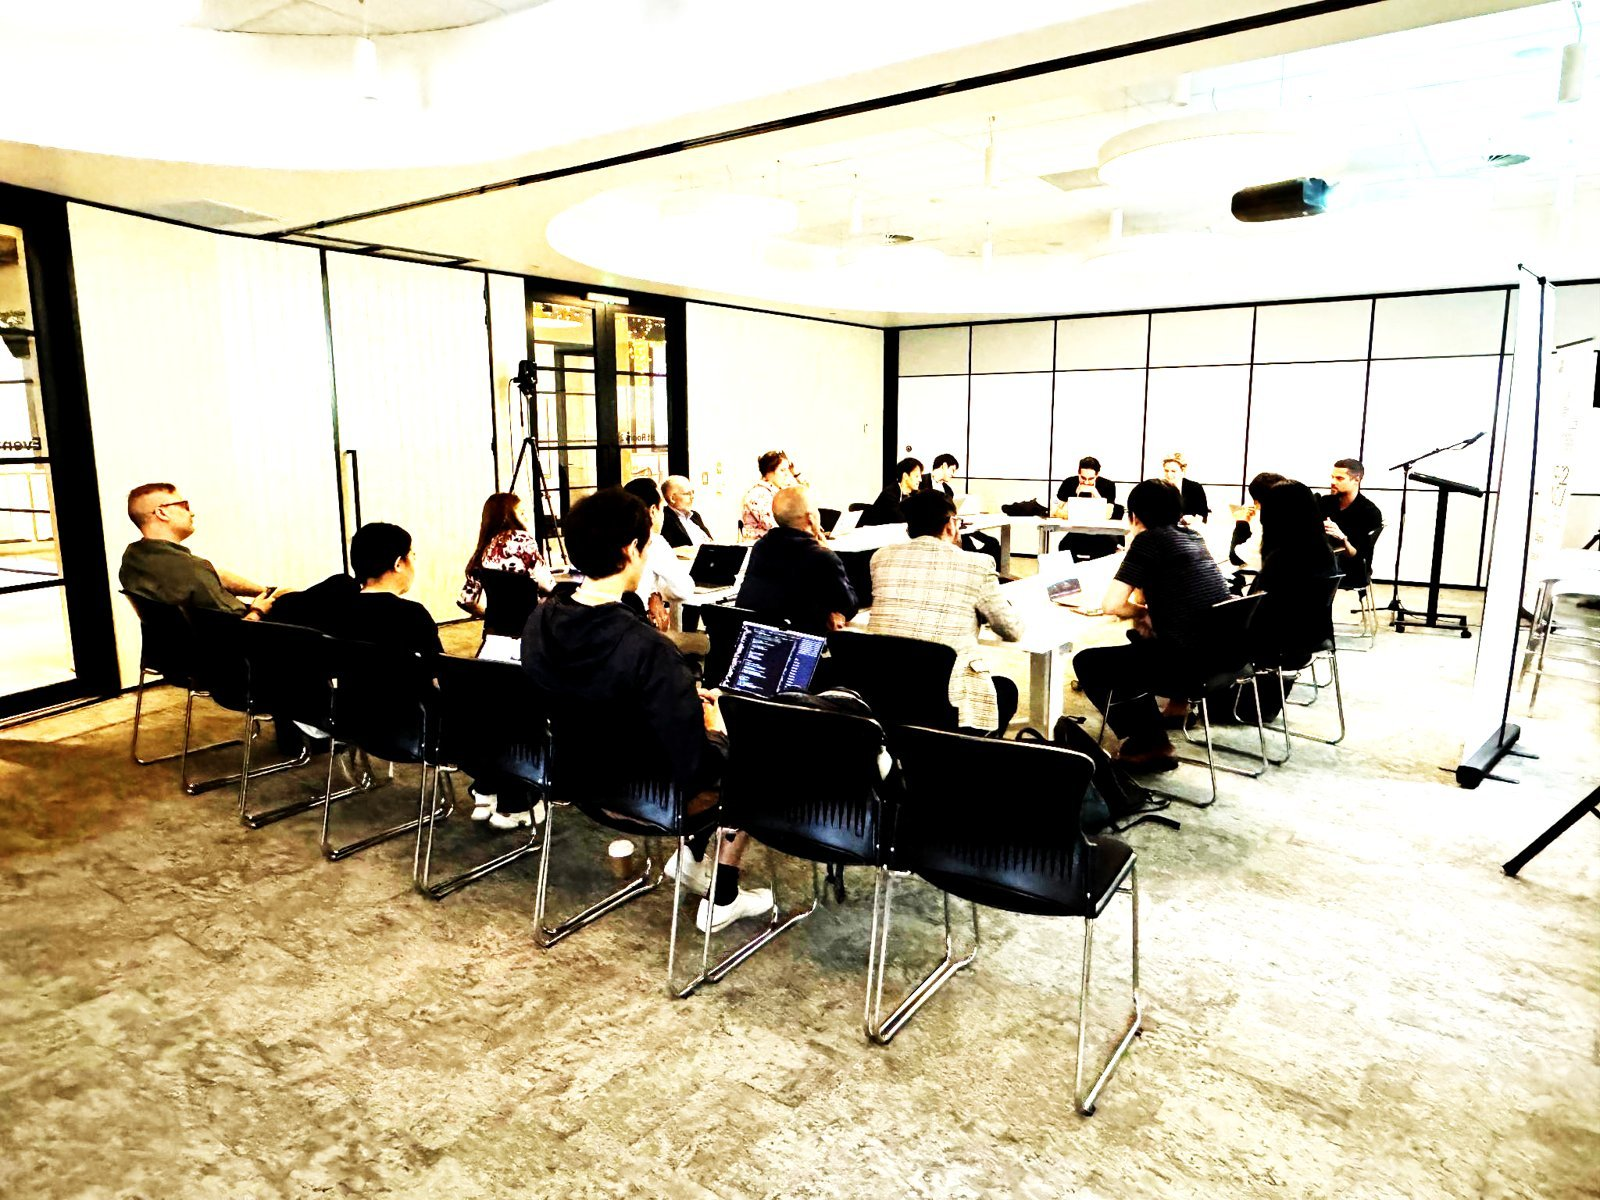
\includegraphics[width=0.49\linewidth]{photo_session1.jpg}\hfill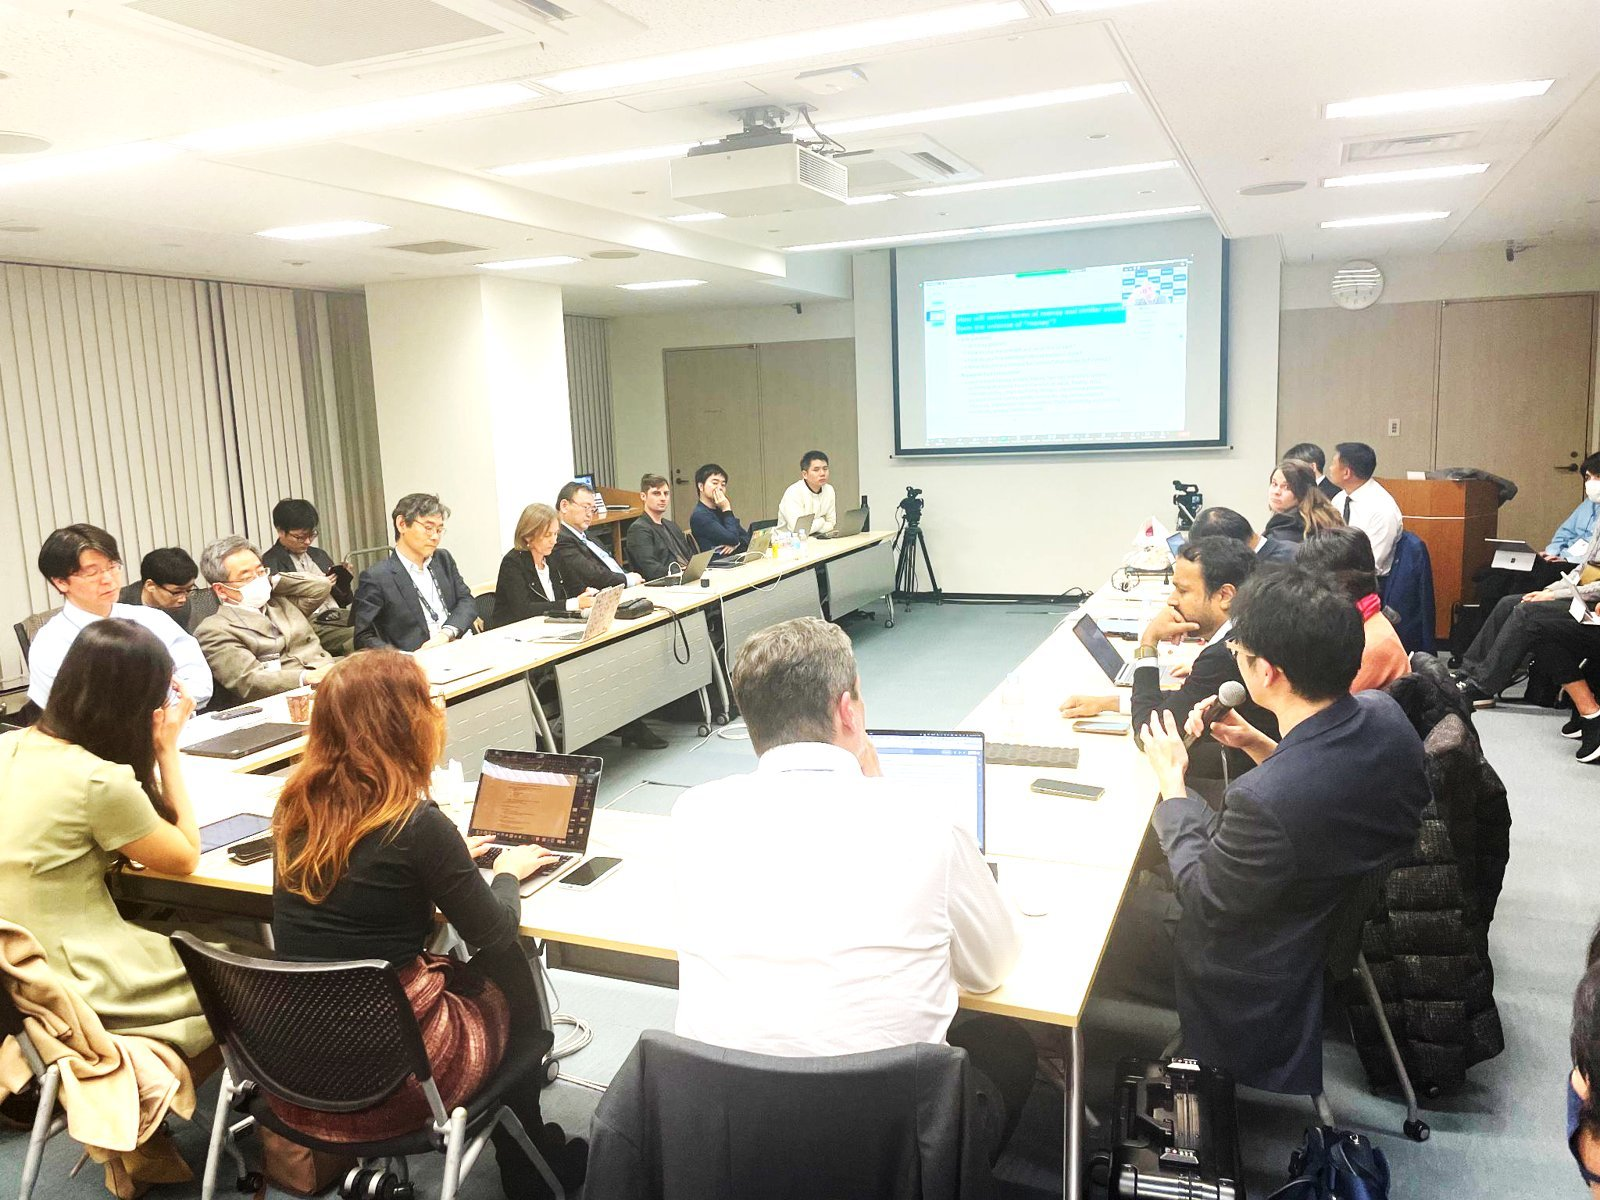
\includegraphics[width=0.49\linewidth]{photo_session2.jpg}\\
      {\scriptsize\color{soft} Prior Block sessions --- multi-stakeholder working format (photos from previous sponsor decks)}
    \end{column}
  \end{columns}
\end{frame}

% ---------------------------------------------------------------- 4 what BGIN provides (image, as-is)
{\setbeamertemplate{footline}{}
\begin{frame}[plain]
  \begin{tikzpicture}[remember picture,overlay]
    \node at (current page.center){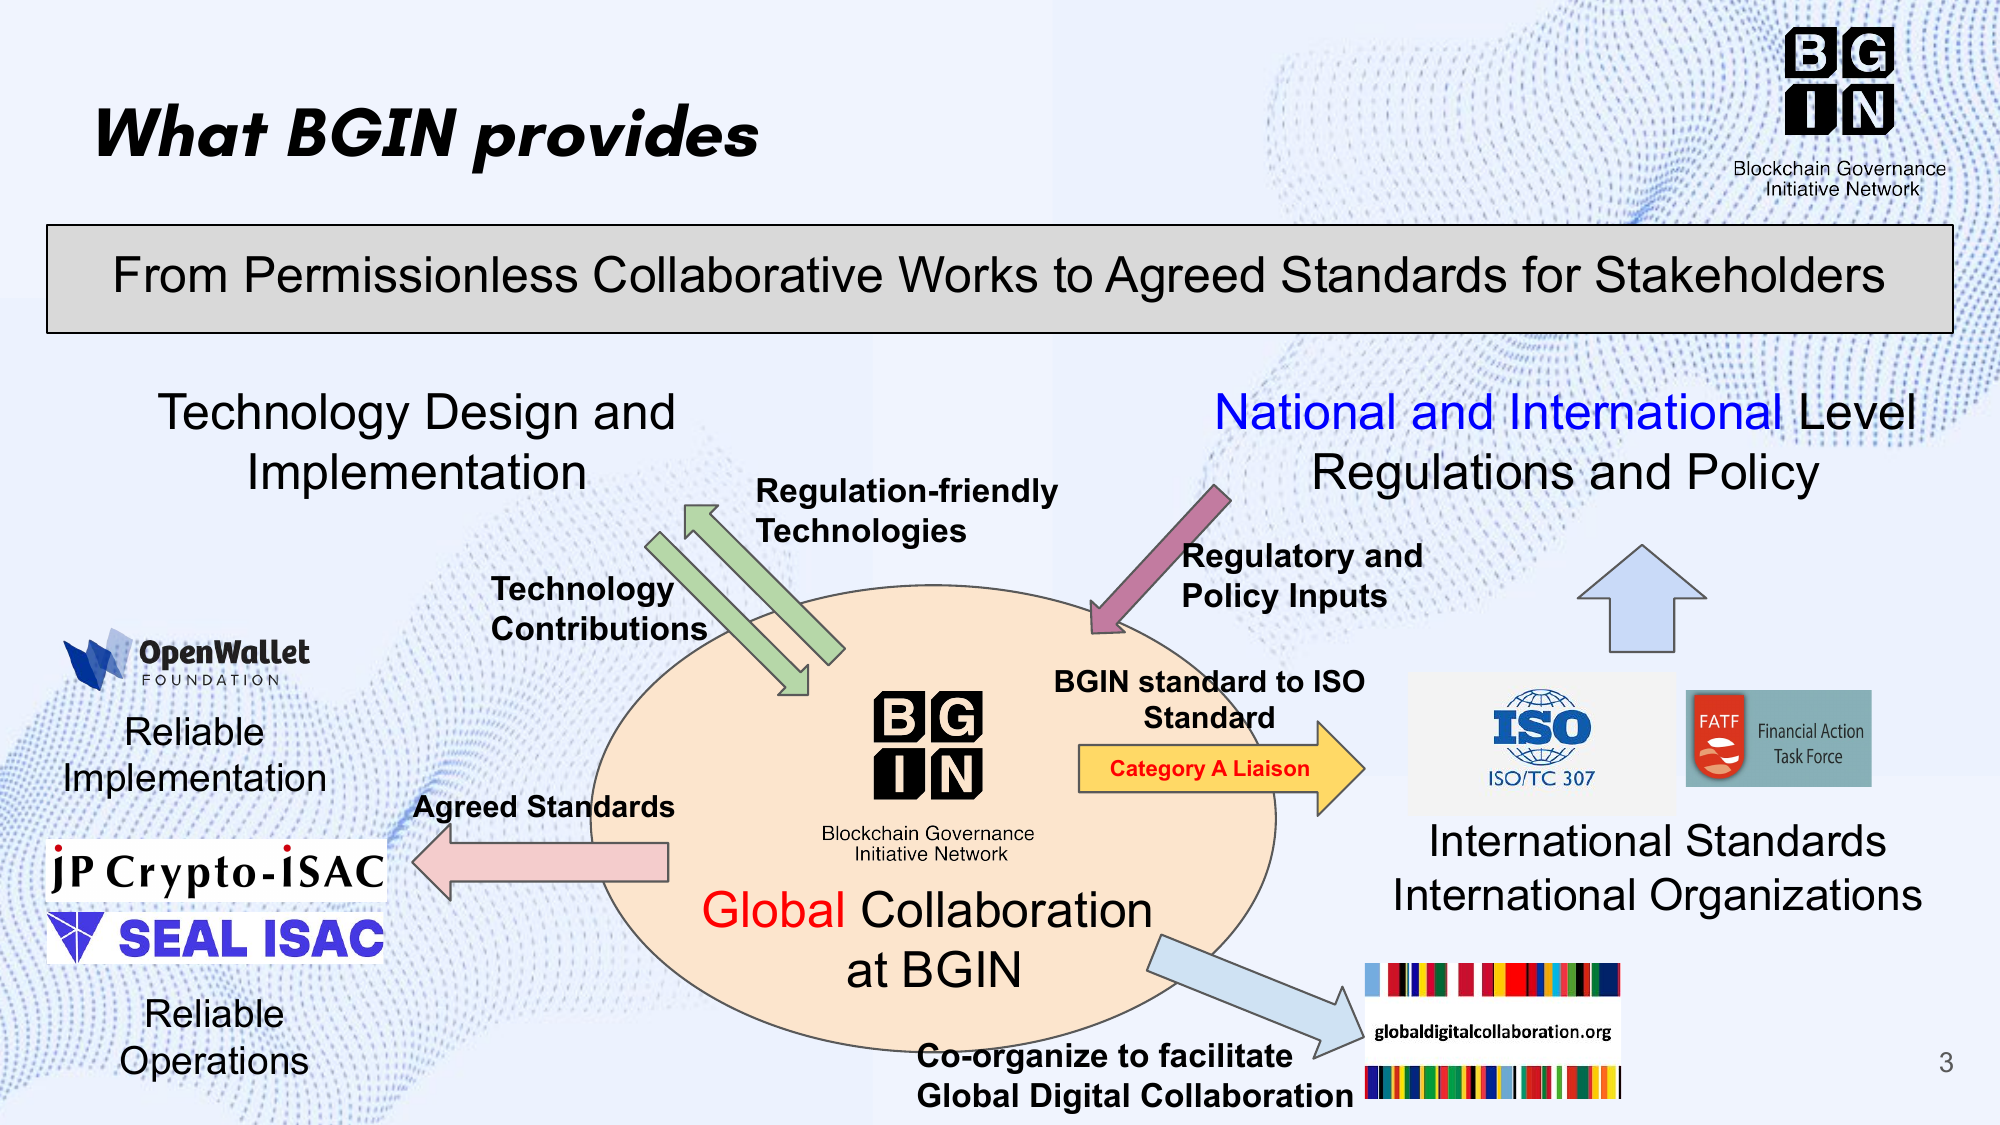
\includegraphics[width=\paperwidth]{what_bgin_provides.png}};
  \end{tikzpicture}
\end{frame}}

% ---------------------------------------------------------------- 5 what sponsors buy
\begin{frame}{What Sponsors Buy}
  \lead{Not inventory for sale --- three outcomes. The legitimacy comes from \textbf{neutral, transparent consensus}: BGIN endorses no chain and no signature scheme, so what it publishes can be cited by everyone.}
  \pillar{Access}{Tickets into the room; introductions to WG chairs and the competition conveners; networking reception presence.}\hfill
  \pillar{Influence}{Tier 1 workshop slot (Day 1 Industry Sessions); a \textbf{technical-advisor seat on the Bitcoin track} --- input on metrics, baselines and the testbed, \emph{without} winner-selection votes; early consolidated meeting report.}\hfill
  \pillar{Association}{Visible support for outputs that carry \textbf{multi-stakeholder legitimacy} --- usable by builders, SROs and government --- unlike one-sided ``self-issued'' papers.}
  \why{Because the process is neutral and transparent, a BGIN metric register or migration standard can be referenced with credibility that a single-project paper lacks --- and Bitcoin's evidence is in it only if Bitcoin engineers put it there.}
\end{frame}

% ---------------------------------------------------------------- 6 NEW: where Bitcoin evidence lands
\begin{frame}{The PQC Migration Track --- Where Bitcoin Evidence Lands}
  {\small
  \begin{tabular}{@{}p{2.6cm}p{11.4cm}@{}}\toprule
    \textbf{Baselines} & B-01 secp256k1 ECDSA (legacy / SegWit v0) \textperiodcentered{} B-02 secp256k1 Schnorr, BIP-340 (Taproot) --- measured for the deltas, not candidates \\
    \textbf{Candidates} & S-01 ML-DSA (FIPS 204) \textperiodcentered{} S-02 SLH-DSA (FIPS 205) \textperiodcentered{} S-03 FN-DSA / Falcon (FIPS 206 draft) \textperiodcentered{} S-04 XMSS \textperiodcentered{} S-05 LMS / HSS (SP 800-208; state handling is \emph{scored}) \\
    \textbf{Paths} & C-01 hybrid classical + PQ (measured as one unit) \textperiodcentered{} C-02 quantum-resistant output type, P2QRH / BIP-360 direction --- reference for the BTC mapping only, \textbf{no endorsement} \\
    \textbf{BTC-tx metrics} & M-05 batch verify \textperiodcentered{} M-07 vbytes / weight per reference block mix \textperiodcentered{} M-08 mempool propagation p50/p95 \textperiodcentered{} M-09 block validation delta on a reference full node \textperiodcentered{} M-11 bytes per UTXO \textperiodcentered{} M-15 wallet / seed / hardware-wallet impact \\
    \textbf{Roadmap} & W2 Block 15 (Oct): committee, rulings \textperiodcentered{} W3 (Nov): harness + result schema, \textbf{node-host call} \textperiodcentered{} W4 SSR (13 Dec): rubric v1, ``PQC-ready chain'' definition, call-text package \textperiodcentered{} W5 (Jan): pilot nodes \textperiodcentered{} W6 CoDecFin 2027 (Feb): standard outline \\
    \bottomrule
  \end{tabular}}
  \why{The testbed exercises \emph{pre-existing} schemes in Bitcoin-mappable configurations with an open harness. Everything above is draft v0 and public --- \href{https://github.com/bgin-global/pqc-agility-competition}{github.com/bgin-global/pqc-agility-competition} --- and the rulings are argued at Block 15.}
\end{frame}

% ---------------------------------------------------------------- 7 day 1
\begin{frame}{Programme --- Day 1 (Thursday 15 October)}
  {\small
  \begin{tabular}{@{}p{2.1cm}p{5.9cm}p{6cm}@{}}\toprule
    \textbf{Time} & \textbf{Room A} & \textbf{Room B / Open Space}\\ \midrule
    09:00--09:20 & Opening Plenary & --- \\
    09:20--09:50 & \textbf{Keynote: PQC} & --- \\
    09:50--11:20 & FASE: AI \& Blockchain & \textbf{IKP: PQC Migration (1)} --- resource estimates and the ECDSA.fail numbers into judging criteria \newline Open Space: Agent Hack / Local Pi Private Knowledge Network \\
    11:30--13:00 & Cyber: Governance of the Security Supply Chain & \textbf{IKP: PQC Migration (2)} --- crypto agility as a governance property; NIST signature migration path, with NIST participation \\
    14:00--14:45 & \textbf{Industry Session 1} & --- \\
    14:45--15:30 & \textbf{Industry Session 2} & --- \\
    15:40--17:10 & BGIN Business Meeting & --- \\
    17:10+ & Networking Reception & --- \\ \bottomrule
  \end{tabular}}
  \why{The two PQC Migration sessions are where the committee is seated and the Bitcoin scheme rulings are argued --- the sessions to attend if only one day is possible. Industry Sessions 1--2 are the published slots for Event Tier 1 / Sustaining workshop activation under BGIN neutrality rules.}
\end{frame}

% ---------------------------------------------------------------- 8 day 2
\begin{frame}{Programme --- Day 2 (Friday 16 October)}
  {\small
  \begin{tabular}{@{}p{2.1cm}p{5.9cm}p{6cm}@{}}\toprule
    \textbf{Time} & \textbf{Room A} & \textbf{Room B}\\ \midrule
    09:00--09:20 & Day 2 Opening & --- \\
    09:20--09:50 & Keynote: Policy & --- \\
    09:50--11:20 & FASE: Industrial Design of Digital Assets & Cyber + IKP: Security AI Agent \\
    11:30--13:00 & FASE: Decentralized Compute \& Market Structure & IKP: Privacy Auth, ZKP \& Proof of Personhood \\
    14:00--14:45 & FASE: Stablecoin Policy --- a Global Outlook & \textbf{Cyber + IKP: Offline Key Management} \\
    15:40--17:10 & AML Policy, Forensics \& Analytics --- Common Taxonomy (FASE/IKP) & Cyber: ST/PP \\ \bottomrule
  \end{tabular}}
  \why{Day 2 is the working depth for a Bitcoin reader: offline / cold key management (where at-rest exposure and key rotation are handled), the security AI agent, and the common taxonomy that operators and analytics vendors will cite.}
\end{frame}

% ---------------------------------------------------------------- 9 tracks
\begin{frame}{Session Tracks --- What a Bitcoin Reader Walks Into}
  {\small
  \begin{tabular}{@{}p{2cm}p{7.4cm}p{4.6cm}@{}}\toprule
    \textbf{Track} & \textbf{Published sessions (Block 15 timetable)} & \textbf{Bitcoin relevance}\\ \midrule
    IKP & \textbf{Keynote: PQC} + two \textbf{PQC Migration} sessions \textperiodcentered{} Privacy Auth, ZKP \& Proof of Personhood \textperiodcentered{} AML / Forensics Common Taxonomy (w/ FASE) & Metric register, baselines B-01/B-02, scheme rulings, testbed node call \\
    Cyber & Governance of the Security Supply Chain \textperiodcentered{} Security AI Agent (w/ IKP) \textperiodcentered{} \textbf{Offline Key Management} \textperiodcentered{} ST/PP & Cold storage, signing-device supply chain, incident sharing \\
    FASE & AI \& Blockchain \textperiodcentered{} Industrial Design of Digital Assets \textperiodcentered{} Decentralized Compute \& Market Structure \textperiodcentered{} Stablecoin Policy \textperiodcentered{} Common Taxonomy (w/ IKP) & Market-structure context; how a migration reads to policy \\
    Agentic AI & Agent Hack / Local Pi Private Knowledge Network (Open Space, Day 1 morning) & Hands-on room; bring a node \\
    General & Opening Plenary \textperiodcentered{} Keynote: Policy \textperiodcentered{} Industry Sessions 1--2 \textperiodcentered{} BGIN Business Meeting \textperiodcentered{} Reception & Sponsor slots; the Block's decisions \\ \bottomrule
  \end{tabular}}
  \why{Priority for Block 15: NIST-facing PQC depth in DC, alongside Industrial Design of Digital Assets and the AML / Forensics Common Taxonomy.}
\end{frame}

% ---------------------------------------------------------------- 10 past partners
\begin{frame}{Past Partners --- Social Proof}
  {\small Organizations that have supported recent Blocks and/or Sustaining programmes include:}\\[2mm]
  \begin{columns}[T]
    \begin{column}{0.62\textwidth}
      {\small\textbf{Event sponsors} (selected, Blocks \#5--\#14)}\\[1mm]
      {\footnotesize Bitbank \textperiodcentered{} Blockchain APAC \textperiodcentered{} Casper Network \textperiodcentered{} Chainalysis \textperiodcentered{} Circle \textperiodcentered{} Coinbase \textperiodcentered{} DeCurret \textperiodcentered{} Digital Garage \textperiodcentered{} Electric Coin Company \textperiodcentered{} EY \textperiodcentered{} Final Aim \textperiodcentered{} Fintech Association Japan \textperiodcentered{} Genesis \textperiodcentered{} Ginco \textperiodcentered{} Hedera \textperiodcentered{} Japan Digital Design \textperiodcentered{} Kraken \textperiodcentered{} Lightlink \textperiodcentered{} Mercari \textperiodcentered{} Monex Group \textperiodcentered{} MUFG \textperiodcentered{} NRI \textperiodcentered{} NTT DATA \textperiodcentered{} NTT Digital \textperiodcentered{} Penguin Securities \textperiodcentered{} Rakuten Wallet \textperiodcentered{} Recruit \textperiodcentered{} SMBC \textperiodcentered{} Soulbis \textperiodcentered{} Swiss Embassy \textperiodcentered{} VerifyVASP \textperiodcentered{} World Foundation}
    \end{column}
    \begin{column}{0.34\textwidth}
      {\small\textbf{Sustaining} (examples)}\\[1mm]
      {\footnotesize Digital Garage \textperiodcentered{} JP Crypto-ISAC}\\[3mm]
      {\small\textbf{Institutional context}}\\[1mm]
      {\footnotesize Liaison: ISO/TC 307 \textperiodcentered{} FATF VACG}
    \end{column}
  \end{columns}
  \why{Exchanges, custodians and analytics firms that carry Bitcoin every day have sponsored before. The protocol-engineering side of Bitcoin has not yet had a named seat in this track --- that is the invitation.}
\end{frame}

% ---------------------------------------------------------------- 11 packages
\begin{frame}{Packages at a Glance}
  {\small\textbf{Event Sponsorship} (per Block)\hfill Tier 1 \$10,000\quad Tier 2 \$5,000\quad Tier 3 \$2,500}\\[1mm]
  {\small\begin{tabular}{@{}p{8cm}ccc@{}}\toprule
    \textbf{Benefit} & T1 & T2 & T3\\ \midrule
    Logo on event web page \& on-site & $\circ$ & $\circ$ & $\circ$\\
    Complimentary admission tickets & 10 & 5 & 3\\
    Workshop / session slot & 1 & --- & ---\\ \bottomrule
  \end{tabular}}\\[4mm]
  {\small\textbf{Sustaining Sponsorship} (annual, 3-year term)\hfill Tier 1 \$50,000\quad Tier 2 \$30,000\quad Tier 3 \$15,000}\\[1mm]
  {\small\begin{tabular}{@{}p{8cm}ccc@{}}\toprule
    \textbf{Benefit} & T1 & T2 & T3\\ \midrule
    Logo on BGIN website; priority advertising & $\circ$ & $\circ$ & $\circ$\\
    Tickets each Block & Unlim. & 5 & 3\\
    Workshop slots each Block & 2 & 1 & ---\\
    Industry Advisory Board seat & 2 & 1 & ---\\ \bottomrule
  \end{tabular}}\\[2mm]
  {\scriptsize\color{soft} Participation without sponsorship is open: registration is public, and fee waivers apply to written contributions presented at the meeting.}
\end{frame}

% ---------------------------------------------------------------- 12 activation
\begin{frame}{Activation Menu --- Beyond the Logo}
  \begin{columns}[T]
    \begin{column}{0.48\textwidth}
      {\small\textbf{Included / tier-linked}}
      \begin{itemize}\small
        \item Workshop slot (Event T1 / Sustaining T1--T2) --- Day 1 Industry Sessions
        \item Complimentary registrations
        \item Web \& on-site recognition
        \item Sustaining: Advisory Board pathway
      \end{itemize}
    \end{column}
    \begin{column}{0.48\textwidth}
      {\small\textbf{\`A la carte / in-kind (examples)}}
      \begin{itemize}\small
        \item Networking Reception --- \$3,000 or in-kind (2 spots)
        \item Coffee / break host
        \item \textbf{Travel support fund} --- brings open-source Bitcoin contributors into the room
        \item \textbf{Testbed node hosting} (in-kind, from W3) --- a reference full node in the neutral testbed
        \item Post-event debrief (15 min) + one-pager metrics
      \end{itemize}
    \end{column}
  \end{columns}
  \vspace{1mm}
  {\small\textbf{Deliverables after Block 15:} session reports to participants; Sustaining sponsors receive the consolidated meeting report (per agreement). The competition record itself is public: decision records, metric register and workshop records land in the repository.}
\end{frame}

% ---------------------------------------------------------------- 13 funds
\begin{frame}{How Funds Are Used}
  \begin{columns}[T]
    \begin{column}{0.48\textwidth}
      {\small\textbf{Event fees \& tickets}}
      \begin{itemize}\small
        \item Venue, catering, AV
        \item Selected travel support (incl. open-source contributors)
        \item Lanyards, banners, materials
        \item Layer 2 meetup support (co-located with Bitcoin and other ecosystem events)
      \end{itemize}
    \end{column}
    \begin{column}{0.48\textwidth}
      {\small\textbf{Sustaining}}
      \begin{itemize}\small
        \item BN (non-profit): operation \& development of BGIN
        \item Surplus supports programmes beyond a single Block
      \end{itemize}
    \end{column}
  \end{columns}
  \why{Steering Committee decisions on fund use are documented for transparency. Sponsorship buys presence and a workshop slot --- it does not buy a vote on the competition's evaluation committee.}
\end{frame}

% ---------------------------------------------------------------- 14 venue
\begin{frame}{Venue}
  \begin{columns}[T]
    \begin{column}{0.5\textwidth}
      \begin{itemize}\small
        \item \textbf{Dates:} 15--16 October 2026\\ Thursday--Friday, same week as DC Fintech Week
        \item \textbf{Venue:} Georgetown University Capitol Campus\\ 111 Massachusetts Avenue NW, Washington, D.C.
        \item \textbf{Format:} Hybrid (in-person encouraged)
        \item \textbf{Event page:} \href{https://bgin-global.org/events/20261015-block15}{bgin-global.org/events/20261015-block15}
        \item \textbf{Registration:} Eventbrite via the event page; fee waivers for written contributions presented at the meeting (submissions close about a week before)
      \end{itemize}
    \end{column}
    \begin{column}{0.46\textwidth}
      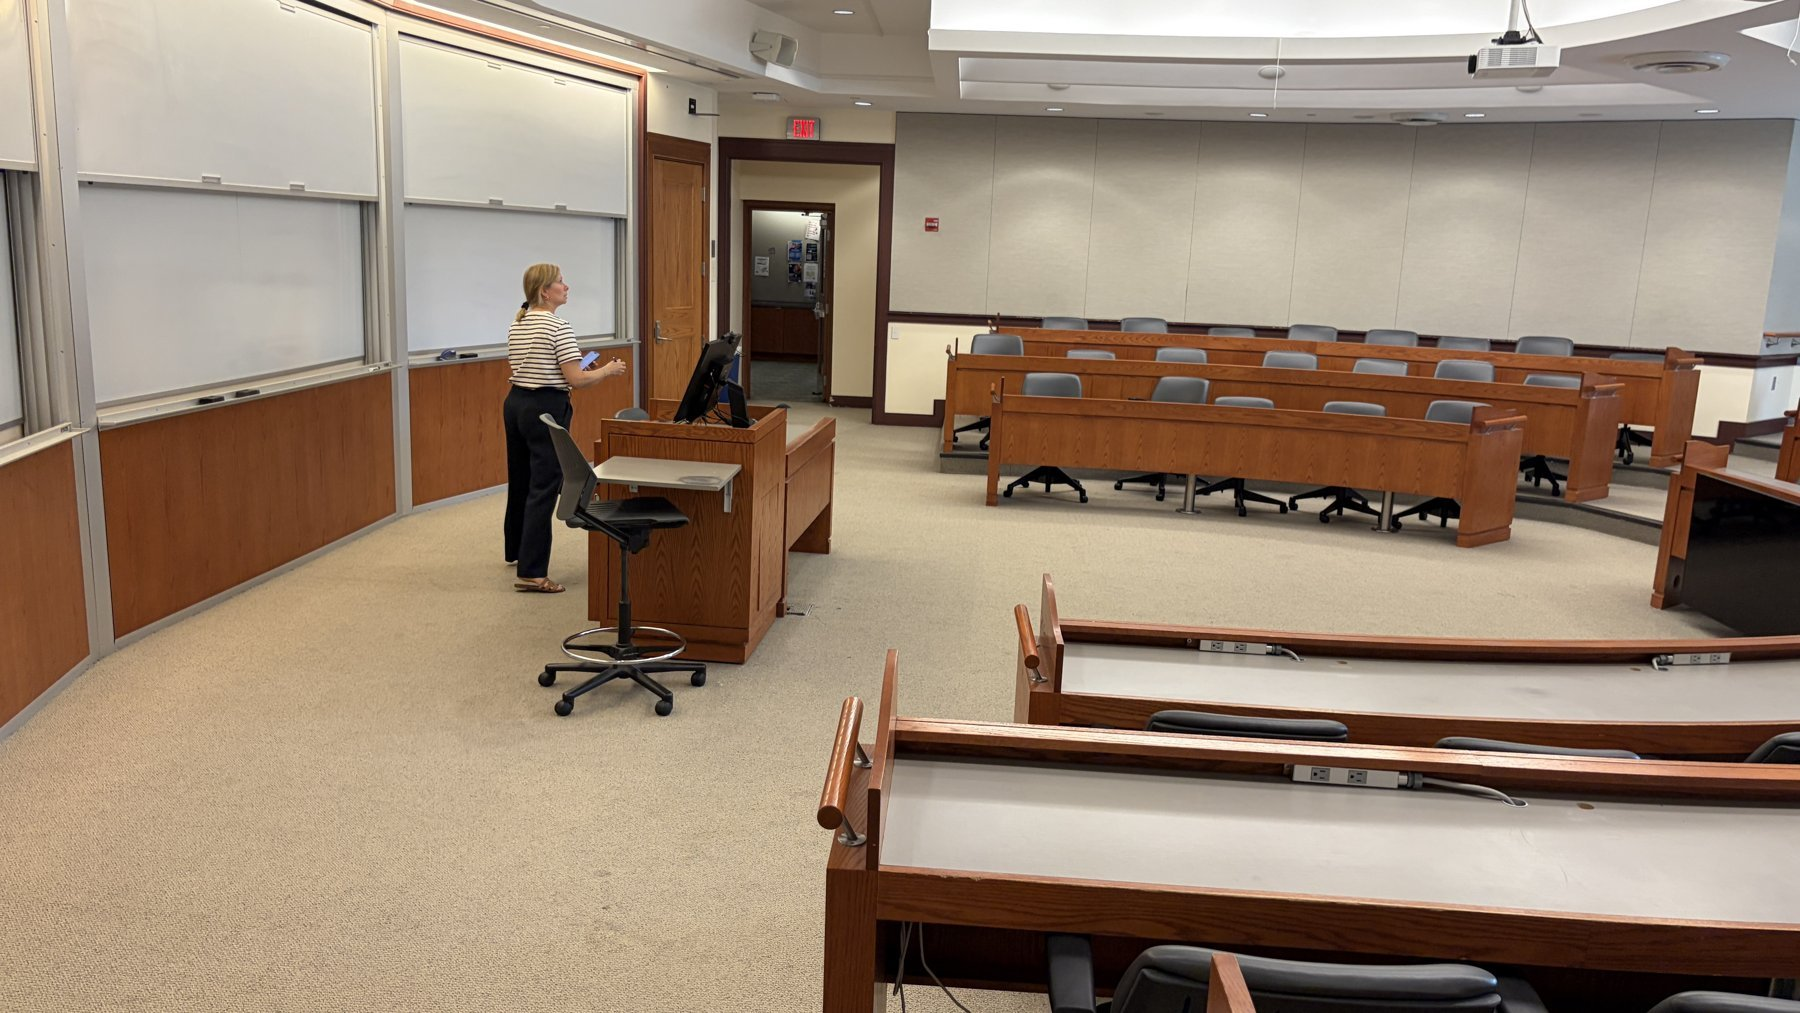
\includegraphics[width=\linewidth]{venue.jpg}\\
      {\scriptsize\color{soft} Venue reference --- Georgetown University}
    \end{column}
  \end{columns}
\end{frame}

% ---------------------------------------------------------------- 15 next steps
\begin{frame}{Next Steps}
  \lead{Two doors. Contributors walk in through the first; sponsors through the second. Reply with a preferred tier and we send the agreement draft and artwork checklist.}
  {\small\textbf{Contribute}}
  \begin{enumerate}\small
    \item \textbf{Register} for Block 15 (fee waiver for a written contribution) and come to the two PQC Migration sessions
    \item \textbf{Open a PR or issue} on the competition repository --- metrics, baselines, the BTC-tx mapping, testbed harness
    \item \textbf{Nominate} a technical advisor for the Bitcoin track (COI form; input without winner votes)
  \end{enumerate}
  {\small\textbf{Sponsor}}
  \begin{enumerate}\small
    \item \textbf{Indicate interest} --- Event Tier 1 / 2 / 3, Sustaining Tier 1 / 2 / 3, and/or Reception / travel fund / node hosting
    \item \textbf{Confirm soon} to lock an Industry Session / workshop slot (programme published; registration open)
    \item \textbf{Artwork \& billing} --- logo files, invoice entity, wire details; optional 15-minute discovery call
  \end{enumerate}
  {\small\textbf{Contact:} BGIN Secretariat --- \href{mailto:bgin_admin@bg2x.org}{bgin\_admin@bg2x.org}\quad\textbf{Repository:} \href{https://github.com/bgin-global/pqc-agility-competition}{github.com/bgin-global/pqc-agility-competition}\quad\textbf{Discussion:} BGIN Discourse, \emph{Post-Quantum Crypto Agility Competition} category}
\end{frame}

% ---------------------------------------------------------------- appendix
\begin{frame}{Appendix --- Who We Are}
  {\small BGIN is a non-profit standardization organization that creates \textbf{neutral forums} for in-depth discussion among all stakeholders --- documenting a common language, exploring innovation and best practices, and advancing standards for blockchain governance in operational, regulatory, and technical spheres.}\\[4mm]
  \begin{columns}[T]
    \begin{column}{0.48\textwidth}
      {\small\textbf{Core stance}}\\[1mm]
      {\small From regulators to cipherpunks \textperiodcentered{} Permissionless participation \textperiodcentered{} Multi-stakeholder consensus}
    \end{column}
    \begin{column}{0.48\textwidth}
      {\small\textbf{Institutional anchors}}\\[1mm]
      {\small ISO/TC 307 Category A Liaison \textperiodcentered{} FATF VACG \textperiodcentered{} IETF-style working practice}
    \end{column}
  \end{columns}
\end{frame}

\begin{frame}{Appendix --- History}
  \begin{columns}[T]
    \begin{column}{0.5\textwidth}
      \begin{itemize}\small
        \item \textbf{2019:} G20 Fukuoka/Osaka --- Communiqu\'e
        \item \textbf{2020:} BGIN launch; Blocks begin worldwide
        \item \textbf{2020--2025:} Blocks \#1--\#12 globally
        \item \textbf{Oct 2025 --- Block 13:} Washington, D.C. (Georgetown)
        \item \textbf{Mar 2026 --- Block 14:} Tokyo (Japan Fintech Week)
        \item \textbf{Sep 2026 --- GDC26:} PQC migration breakout; scene-setting by Google Quantum AI
        \item \textbf{Oct 2026 --- Block 15:} Return to Washington, D.C.
      \end{itemize}
    \end{column}
    \begin{column}{0.46\textwidth}
      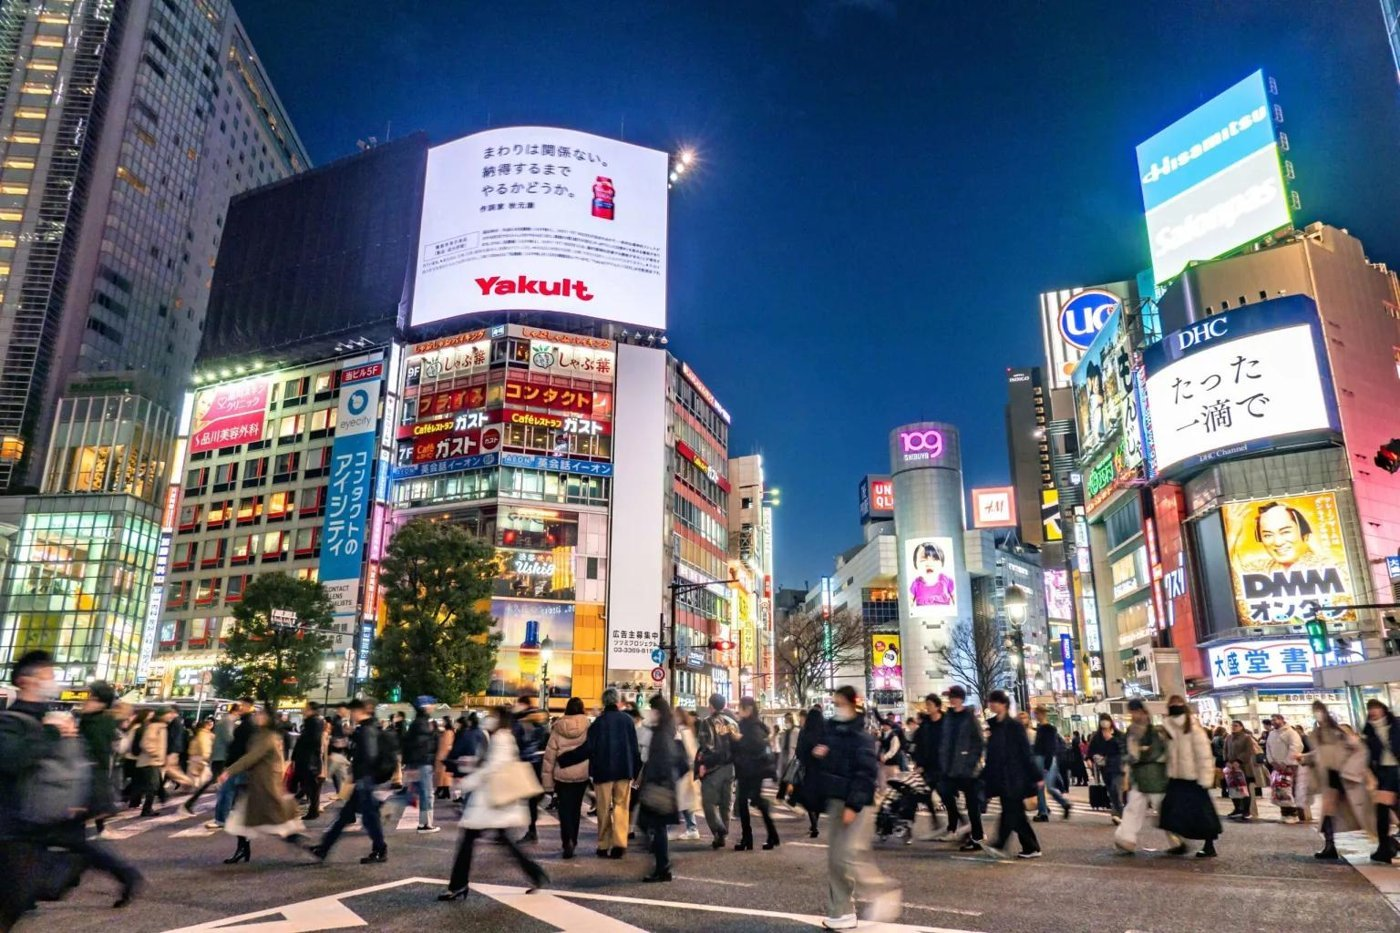
\includegraphics[width=\linewidth]{block14.jpg}\\
      {\scriptsize\color{soft} Block 14 context --- Shibuya, Tokyo (from prior sponsor deck)}
    \end{column}
  \end{columns}
\end{frame}

\begin{frame}{Appendix --- What We Create}
  \begin{columns}[T]
    \begin{column}{0.48\textwidth}
      {\small\textbf{Published} (examples)}
      \begin{itemize}\small
        \item DeFi disclosure \& regulatory considerations
        \item Ransomware reaction; NFT / SBT studies
        \item Decentralized custody incident response
        \item Selective disclosure; stablecoin / DeFi failure points
      \end{itemize}
    \end{column}
    \begin{column}{0.48\textwidth}
      {\small\textbf{Work in progress} --- priorities}
      \begin{itemize}\small
        \item \textbf{Crypto agility \& PQC migration} --- metric register, testbed, ``PQC-ready chain'' definition
        \item Cryptoasset Industry Structure Analysis
        \item Illicit / Unfair Trading Dictionary (common lexicon)
        \item Cybersecurity Information Sharing $\rightarrow$ ISO PAS
        \item ST/PP; Accountable Wallet
        \item AI-assisted security information sharing agent
      \end{itemize}
    \end{column}
  \end{columns}
  {\small\href{https://bgin-global.org/documents}{https://bgin-global.org/documents}}
\end{frame}

{\setbeamertemplate{footline}{}
\begin{frame}[plain]
  \begin{tikzpicture}[remember picture,overlay]
    \node at (current page.center){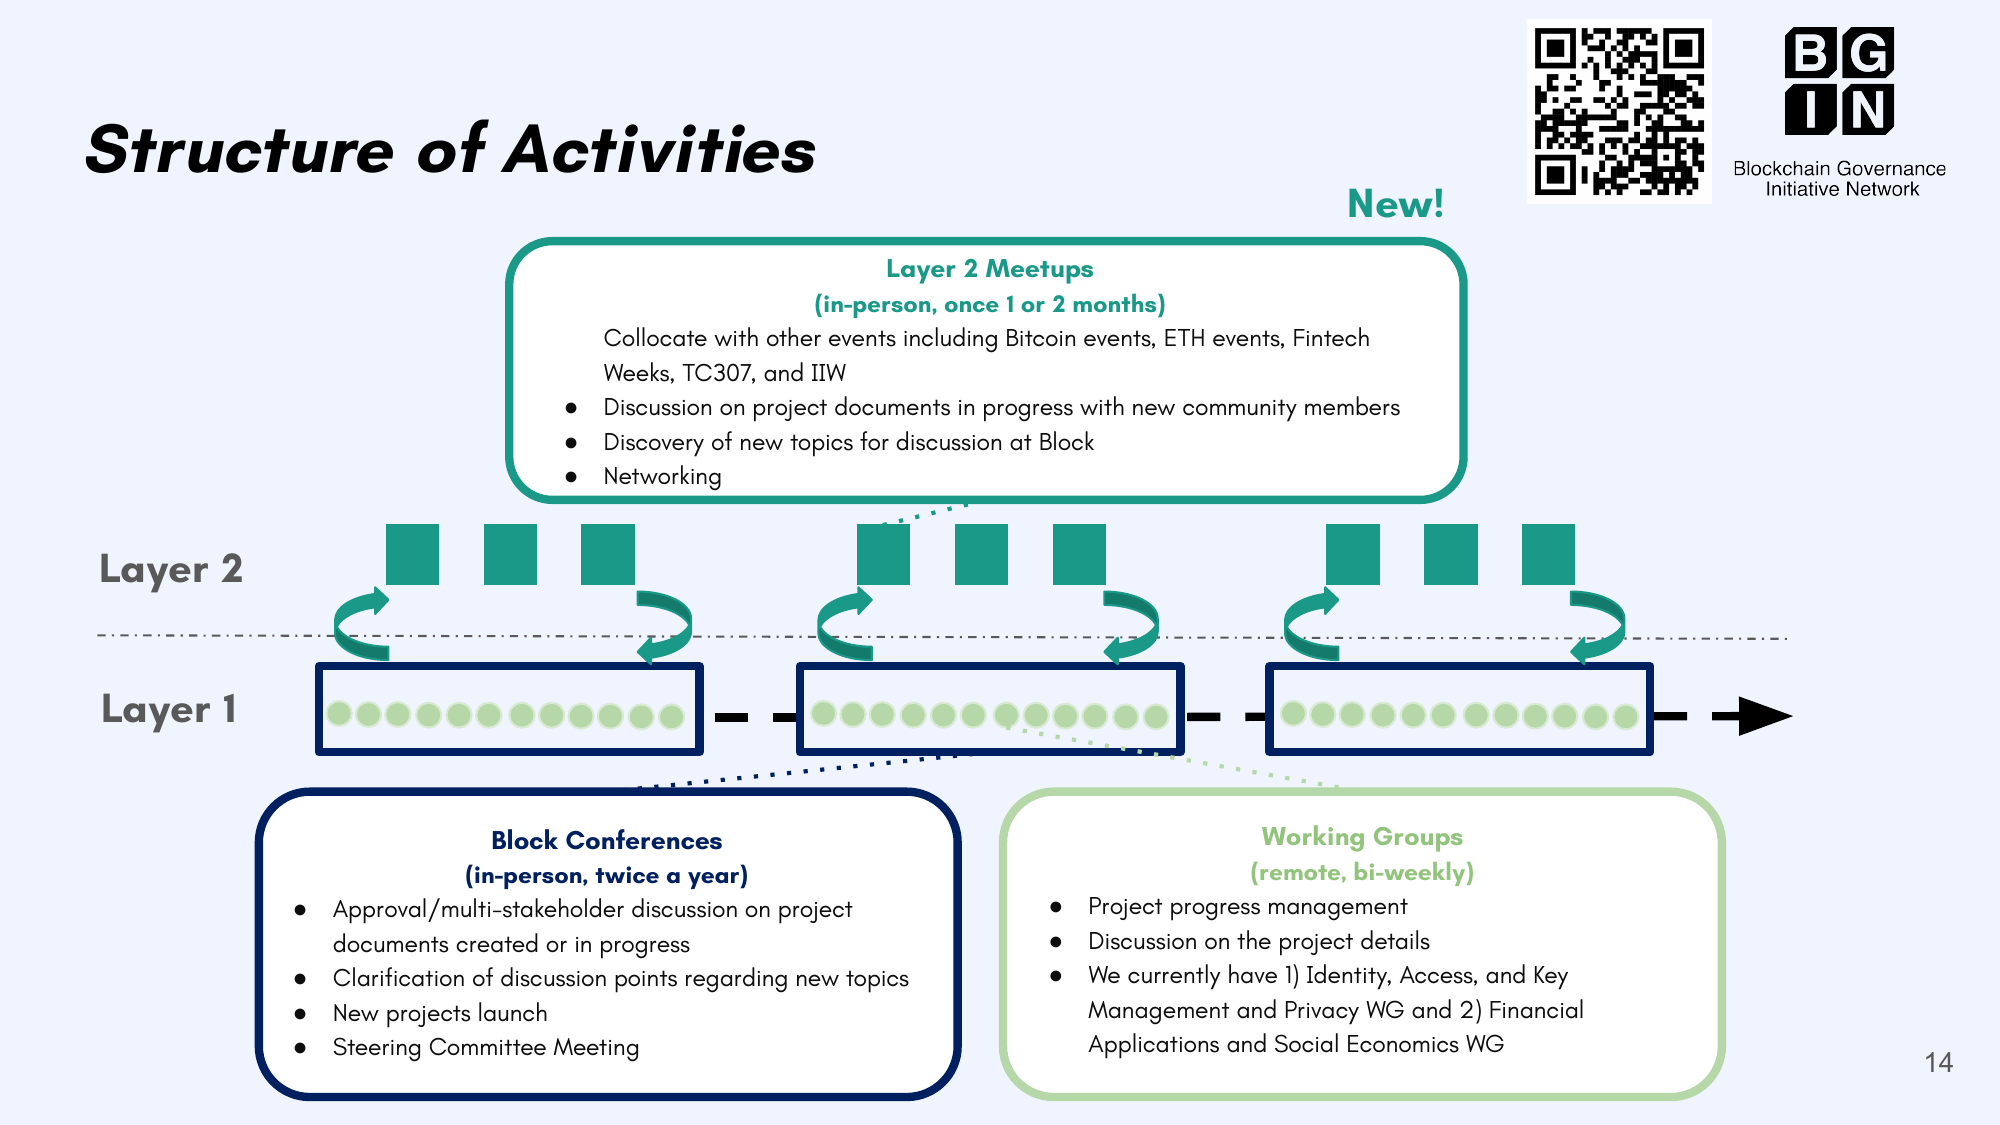
\includegraphics[width=\paperwidth]{structure_of_activities.png}};
    \node[anchor=south west,fill=white,fill opacity=0.85,text opacity=1,font=\scriptsize,text=soft,inner sep=2pt] at ([xshift=4mm,yshift=3mm]current page.south west){Partnerships: ISO/TC 307 \textperiodcentered{} FATF VACG \textperiodcentered{} OpenWallet Foundation \textperiodcentered{} NIST / MITRE / ISACs (session-level). Diagram reused as-is from prior decks; current WGs also include Cyber Security and Agent.};
  \end{tikzpicture}
\end{frame}}

\begin{frame}{Appendix --- Governance}
  \begin{itemize}\small
    \item \textbf{BN Corporation (non-profit)} --- legal, financial, accounting, labor
    \item \textbf{Steering Committee} --- strategy, projects, use of BN funds
    \item \textbf{Industry Advisory Board} --- recommendations to the SC
    \item \textbf{Program Committee} --- Block agenda
    \item \textbf{Working Groups} --- detailed project work
    \item \textbf{Secretary Office} --- operational support
  \end{itemize}
  {\small Roles are specified in BGIN's Bylaws. SC decision-making is shared publicly. The PQC competition adds its own evaluation committee with a published conflict-of-interest policy; sponsorship and committee seats are separate.}
\end{frame}

\begin{frame}{Appendix --- Administration}
  \begin{columns}[T]
    \begin{column}{0.48\textwidth}
      {\small\textbf{Co-Chairs}}\\[0.5mm]
      {\small Shin'ichiro Matsuo (Virginia Tech \& Georgetown)\\ Amanda Wick (ex-US Department of Justice)}\\[3mm]
      {\small\textbf{Working Group Chairs}}\\[0.5mm]
      {\small \textbf{IKP} --- Nat Sakimura \textperiodcentered{} Mitchell Travers\\ \textbf{FASE} --- Chloe White \textperiodcentered{} Joseph Beverley\\ \textbf{Cyber} --- Julien Bringer (Acting)\\ \textbf{Agent} --- Mitchell Travers}
    \end{column}
    \begin{column}{0.48\textwidth}
      {\small\textbf{Steering Committee}}\\[0.5mm]
      {\small Co-Chair Shin'ichiro Matsuo\\ Co-Chair Amanda Wick\\ Ali Nejadmalayeri (University of Wyoming)\\ Roman Pavlov (Individual Engineer)\\ Tomofumi Okubo (Penguin Securities)\\ Julien Bringer (ISO/TC 307 JWG4)\\ Jarek Nabrzyski (University of Notre Dame)\\ Observer: Yuta Takanashi (FSB/JFSA)}
    \end{column}
  \end{columns}
\end{frame}

{\setbeamertemplate{footline}{}
\begin{frame}[plain]
  \begin{tikzpicture}[remember picture,overlay]
    \node at (current page.center){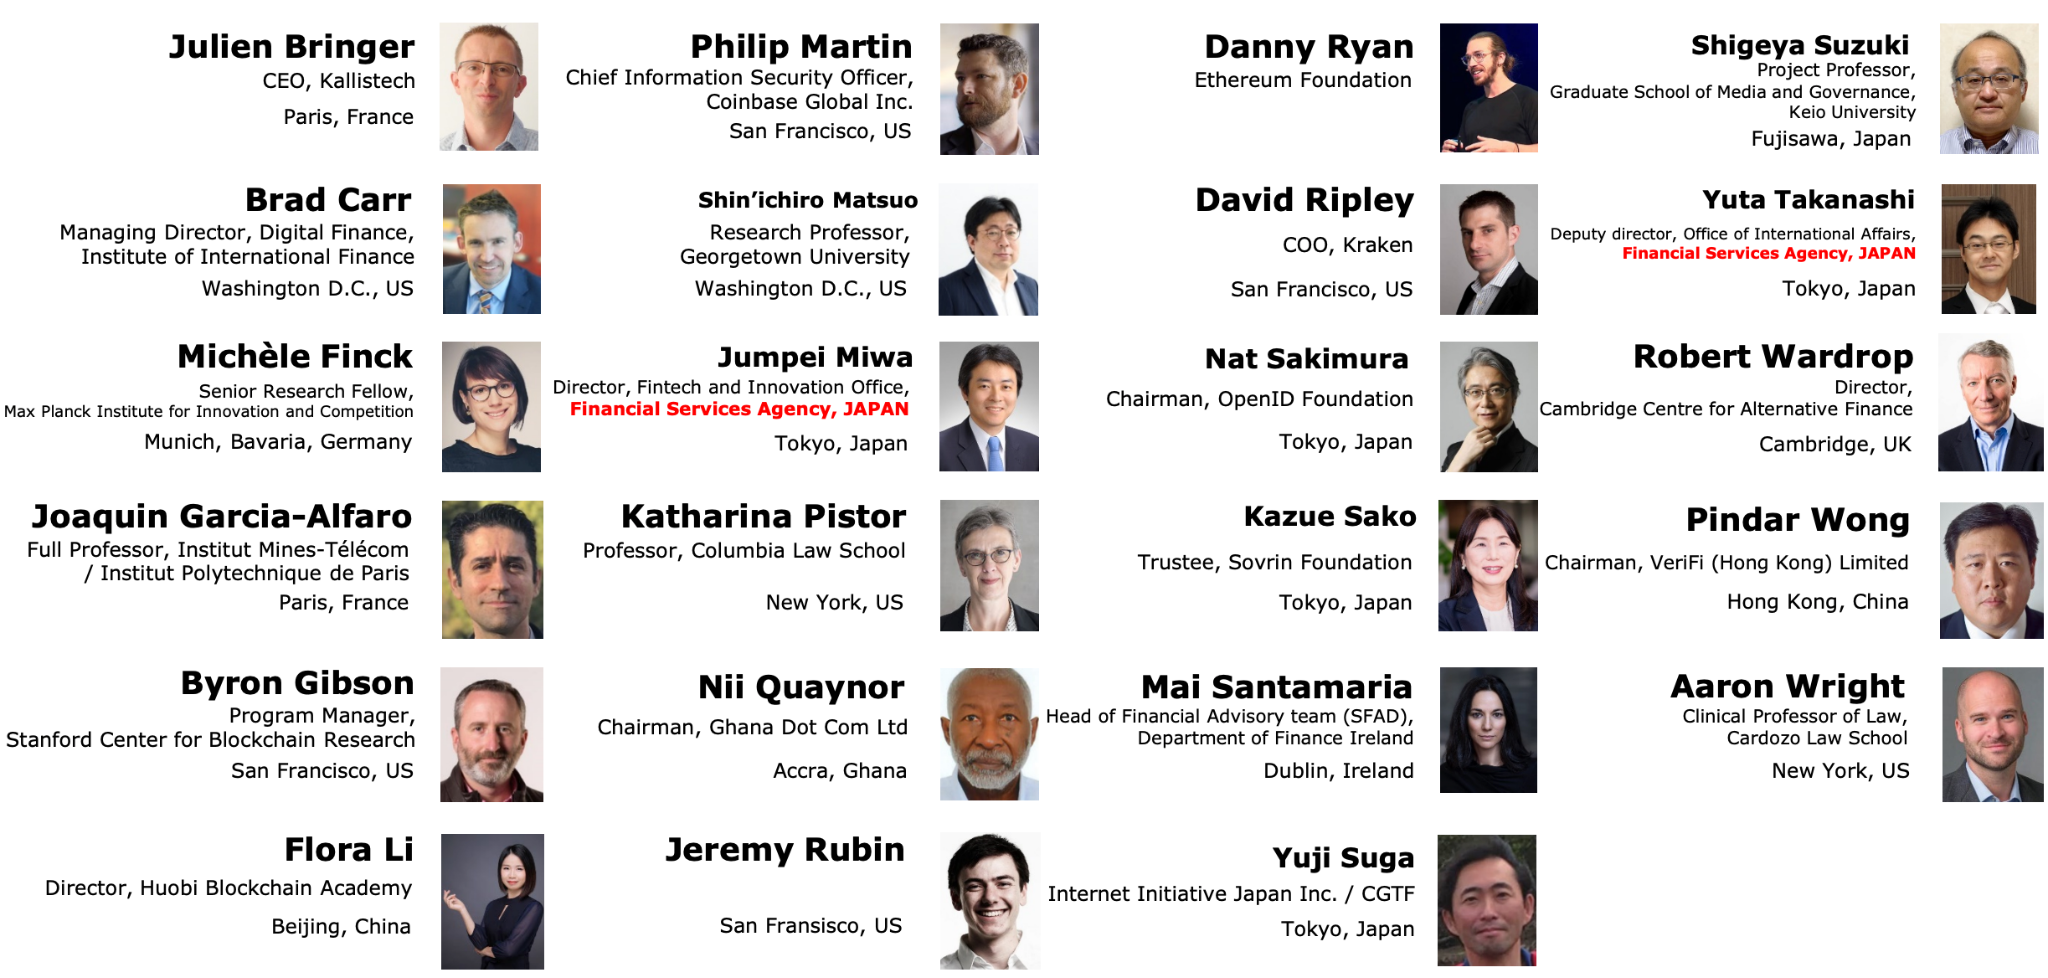
\includegraphics[width=\paperwidth]{initial_contributors.png}};
    \node[anchor=south,fill=white,fill opacity=0.85,text opacity=1,font=\scriptsize,text=soft,inner sep=2pt] at ([yshift=3mm]current page.south){Appendix --- Initial Contributors: multi-stakeholder founding cohort (industry, academia, civil society, and public authorities).};
  \end{tikzpicture}
\end{frame}}

{\setbeamertemplate{footline}{}
\begin{frame}[plain]
  \begin{tikzpicture}[remember picture,overlay]
    \fill[bar] (current page.north west) rectangle (current page.south east);
    \node[anchor=center,text=white,font=\Large\bfseries] at ([yshift=8mm]current page.center){Thank you};
    \node[anchor=center,text=white,font=\small] at ([yshift=-2mm]current page.center){Partner with us for BGIN Block 15 --- bgin\_admin@bg2x.org};
    \node[anchor=center,text=white,font=\small] at ([yshift=-9mm]current page.center){\faGlobe~https://bgin-global.org/ \quad \faGithub~github.com/bgin-global/pqc-agility-competition};
    \node[anchor=south east,inner sep=0] at ([xshift=-7mm,yshift=5mm]current page.south east){
\includegraphics[height=1cm]{bgin_wordmark.png}};
  \end{tikzpicture}
\end{frame}}

\end{document}
